\documentclass[12pt,a4paper]{article}
\usepackage{graphicx} % Required for inserting images
\usepackage{tikz}
\usepackage[left=2.00cm, right=1.00cm]{geometry}
\usepackage{xcolor} % before tikz or tkz-euclide if necessary
\usepackage{amsmath}
\usepackage{siunitx}
\usepackage{chemfig}
\usetikzlibrary{calc}
\usepackage[english]{babel}
\begin{document}
\begin{center}
    \large\textbf{Test in Thermodynamics:}
\end{center}
1. How is the Kelvin temperature scale defined?\\\\
2. What is meant by the absolute zero point?\\\\
3. What does the ideal gas law state, and what are the units of the various quantities?\\\\
4. Convert to Kelvin: $35 ^\circ C, 63^\circ C, -26^\circ C, 253^\circ C $\\\\
5. Convert to Celsius: 273.15K, 233K, 57K, 800K\\\\
6. A gas enclosed in a container has a pressure of $P_1=5.3bar$. What will the pressure be when we halve the volume and the temperature remains constant? $V_1=6L$\\\\
7. We are given the following piston containing a gas. We have a piston that can be pushed in and out:\vspace{0.5cm}\\
\begin{center}
    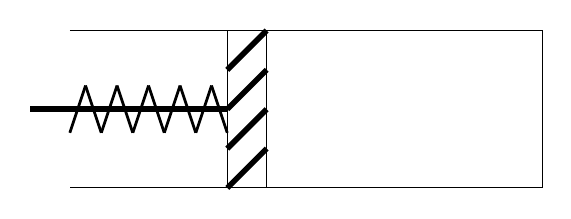
\begin{tikzpicture}
        % piston with variable
        \pgfmathsetmacro{\myLength}{4}
        \draw (2,2)--(8,2)--(8,0)--(2,0);
        \draw (\myLength,0)--(\myLength+0.5,0)--(\myLength+0.5,2)--(\myLength,2)--(\myLength,0);
        \draw [line width=2pt] (\myLength,0)--(\myLength+0.5,0.5);
        \draw [line width=2pt] (\myLength,0.5)--(\myLength+0.5,1);
        \draw [line width=2pt] (\myLength,1)--(\myLength+0.5,1.5);
        \draw [line width=2pt] (\myLength,1.5)--(\myLength+0.5,2);
        \draw [line width=2pt] (\myLength,1)--(\myLength-2.5,1);
        \draw [line width=1pt] (2,0.7)--(2.2,1.3);
        \draw [line width=1pt] (2.2,1.3)--(2.4,0.7);
        \draw [line width=1pt] (2.4,0.7)--(2.6,1.3);
        \draw [line width=1pt] (2.6,1.3)--(2.8,0.7);
        \draw [line width=1pt] (2.8,0.7)--(3.0,1.3);
        \draw [line width=1pt] (3.0,1.3)--(3.2,0.7);
        \draw [line width=1pt] (3.2,0.7)--(3.4,1.3);
        \draw [line width=1pt] (3.4,1.3)--(3.6,0.7);
        \draw [line width=1pt] (\myLength-0.4,0.7)--(\myLength-0.2,1.3);
        \draw [line width=1pt] (\myLength-0.2,1.3)--(\myLength,0.7);
    \end{tikzpicture}
\end{center}\vspace{1cm}
Initially, the volume is $V_1=8L$ and the pressure is $P_1=2.1bar$. We change the volume while the temperature remains constant so that the new volume is $V_2=2L$. What will the new pressure $P_2$ be? \\\\
8. The temperature of a gas is now $T_2=52^\circ C$. We increase the temperature to $T_3=400K$. What will the new pressure $P_3$ be if we assume that the volume is constant?\newpage
We can look at a square block resting on a table:\\\\\\\
\begin{center}
    \begin{tikzpicture}[scale=0.8]
        \draw (4,0)--(4,4);
        \draw (2,4)--(10,4);
        \draw (8,0)--(8,4);
        \draw (5,4) rectangle (7,6);
    \end{tikzpicture}    
\end{center}
This block has a mass (in kg) and a surface area in contact with the table. It therefore exerts a pressure $P$ on the table. The sides have a length of 30cm (0.3m), height of 15cm (0.15m), and width of 20cm (0.2m):\\
\begin{tikzpicture}[scale=1.5,transform canvas={shift={(6cm,-3cm)}}]

% Dimensions
\def\L{4}
\def\B{2}
\def\H{1}

% Depth vector (perspective)
\coordinate (D) at (-0.5,0.3);

% Bottom face
\draw (0,0) -- (\L,0) -- ++(D) -- ++(-\L,0) -- cycle;

% Vertical edges (height)
\draw (0,0) -- ++(0,\H);
\draw (\L,0) -- ++(0,\H);
\draw ($(0,0)+ (D)$) -- ++(0,\H);
\draw ($( \L,0) + (D)$) -- ++(0,\H);

% Top face
\draw (0,\H) -- (\L,\H) -- ++(D) -- ++(-\L,0) -- cycle;

% Depth lines
\draw (\L,0) -- ++(D);
\draw (\L,\H) -- ++(D);
\node at (2,1.5) {length = 30cm (0.3m)};
\node at (5.5,0.5) {height = 15cm (0.15m)};
\node at (-1.8,0.2) {width = 20cm (0.2m)};
\end{tikzpicture}\\
\vspace{4cm}
\\This block can be placed on the table in three different ways. Calculate the three different pressures the block exerts on the table surface.\\
Hint:
$$P=\frac{G}{A}$$
$G=m\cdot g$\\
G = gravitational force (N)\\
m = mass of the block (kg)\\
g = acceleration due to gravity ($m/s^2$)\\
P = pressure on the table surface $(N/m^2, Pa)$\\
A = area of the block in contact with the table ($m^2$)\newpage
\noindent\large\textbf{Useful formulas:}\\\\
Conversion between Kelvin and Celsius:\\
$T_K=T_C+273.15$\\
$T_C=T_K-273.15$\\\\
The ideal gas law:\\\\
$P\cdot V=n\cdot R\cdot T$\\\\
Where:\\\\
P = gas pressure (Pa, $N/m^2$)\\
n = number of molecules, or amount of substance (mol)\\
R = gas constant (8.314J/molK)\\
V = gas volume ($m^3$)\\
T = temperature in K (kelvin)\newpage
\noindent\large\textbf{Gas laws:}\\\\
\textbf{At constant temperature:}\\\\
$$P_1\cdot V_1=P_2\cdot V_2$$
P = pressure (bar or Pa)\\
V = volume (mL or L)\\\\
\textbf{"Cross" form of the formula:}\vspace{1cm}
\begin{center}
    \begin{tikzpicture}
        \draw (0,0) -- (4,0);
        \draw (2,-2) -- (2,2);
        \node at (4.4,0) {$V_1$};
        \node at (-0.4,0) {$P_1$};
        \node at (2,2.4) {$P_2$};
        \node at (2.1,-2.4) {$V_2$};
    \end{tikzpicture}
\end{center}
\textbf{At constant pressure:}\\\\
$$\frac{V_1}{T_1}=\frac{V_2}{T_2}$$\\
T = temperature (NOTE! Must be in Kelvin)\\
V = volume (mL or L)\newpage
\textbf{"Cross" form of the formula:}\vspace{1cm}
\begin{center}
    \begin{tikzpicture}
        \draw (0,0) -- (4,0);
        \draw (2,-2) -- (2,2);
        \node at (4.4,0) {$T_2$};
        \node at (-0.4,0) {$V_1$};
        \node at (2,2.4) {$V_2$};
        \node at (2.1,-2.4) {$T_1$};
    \end{tikzpicture}
\end{center}
\textbf{At constant volume:}\\\\
$$\frac{P_1}{T_1}=\frac{P_2}{T_2}$$\\
P = pressure (bar or Pa)\\
V = volume (mL or L)\\\\
\textbf{"Cross" form of the formula:}\vspace{1cm}
\begin{center}
    \begin{tikzpicture}
        \draw (0,0) -- (4,0);
        \draw (2,-2) -- (2,2);
        \node at (4.4,0) {$T_2$};
        \node at (-0.4,0) {$P_1$};
        \node at (2,2.4) {$P_2$};
        \node at (2.1,-2.4) {$T_1$};
    \end{tikzpicture}
\end{center}

\end{document}